%%%%%%%%%%%%%%%%%%%%%%%%%%%%%%%%%%%%%%%%%%%%%%%%%%%%%%%%%%%%%%
%% LaTeX template for the scientific justification to be       %%
%%     submitted as part of a regular ALMA proposal.        %%
%% This template should also be used for a ToO, Solar, or   %%
%%     mm-VLBI ALMA proposal, but NOT for Large Programs    %%
%%     (these have a separate template with more sections)  %%
%%                                                          %%
%%                      ALMA Cycle 4                        %%
%%                                                          %%
%%%%%%%%%%%%%%%%%%%%%%%%%%%%%%%%%%%%%%%%%%%%%%%%%%%%%%%%%%%%%%

%%%%%%%%%%%%%%%%%%%%%%%%%%%%%%%%%%%%%%%%%%%%%%%%%%
%%%%% How to convert this document to PDF %%%%%%%%
%%%%%%%%%%%%%%%%%%%%%%%%%%%%%%%%%%%%%%%%%%%%%%%%%%

% If your figures are stored as PostScript files, you can use the 
% following commands to generate a PDF file of your proposal:

%% latex file.tex
%% dvips file.dvi
%% ps2pdf file.ps file.pdf 


% If your figures are PDF images or bitmap pictures in PNG, JPG, or GIF format,
% you can use the pdflatex command to generate a PDF file from this template
% (note, however, that the pdflatex command does not handle PostScript files):

% pdflatex file.tex


% WARNINGS: 
%           1. You must make sure that PDF output generated from this
%              template is complete both when displayed with a viewer 
%              (acroread, for example) and when printed on paper.
%              LaTeX installations vary greatly and therefore it might 
%              not be possible to get all proposals to come out 
%              correctly with a single text page layout. 
%              In some cases you will have to adjust the 
%              \topmargin=-7mm command in the template to center the 
%              text vertically in the page.  
%           2. The scientific justification, figures, tables, references,
%              and public outreach statement must all fit within the
%              4-page limit.
%           3. You are free to include color images in your proposal 
%              justification. Proposals are distributed to ALMA Review Panels 
%              in electronic form. However, the scientific content of the 
%              images should still remain clear when displayed or printed
%              in black and white.
%           4. this template is for regular, ToO, Solar, or mm-VLBI ALMA proposals,
%              but NOT for Large Programs: these have a separate template with
%              more sections, and is available from the ALMA Science Portal


%%%%%%%%%%%%%%%%%%%%%%%%%%%%%%%%%%%%%%%%%%%%%%
%%%%% Default format: 12pt single column %%%%%
%% 12pt is the minimum font size allowed !! %%
%%%%%%%%%%%%%%%%%%%%%%%%%%%%%%%%%%%%%%%%%%%%%%

\documentclass[11pt,a4paper]{article}  %% DO NOT CHANGE to 11pt or less !

\usepackage{graphics,graphicx}
\usepackage[T1]{fontenc}
%%%%%%%%%%%%%%%%%%%%%%%%%%%%
%%%%%% Page dimensions %%%%%
%%%%%%  DO NOT CHANGE  %%%%%
%%%%%%%%%%%%%%%%%%%%%%%%%%%%
\newcommand{\alexie}[1]{\textcolor{blue}{\textbf{[Alexie: #1]}}}

\newcommand{\enia}[1]{\textcolor{orange}{\textbf{[Enia: #1]}}}

\newcommand{\later}[1]{\textcolor{magenta}{To be written later. }}
\newcommand{\writenow}[1]{\textcolor{magenta}{Complete this section. #1 }}

\newcommand{\bene}[1]{\textcolor{magenta}{Benedikt please check here}}

\newcommand{\benedikt}[1]{\textcolor{green}{\textbf{[Benedikt: #1]}}}



\textheight=260mm
\textwidth=180mm
\topmargin=-20mm
\oddsidemargin=-10mm
\evensidemargin=-10mm
\parindent 10pt

%%%%%%%%%%%%%%%%%%%%%%%%%%%%%
%%%%% Start of document %%%%% 
%%%%%%%%%%%%%%%%%%%%%%%%%%%%%

\begin{document}
\pagestyle{plain}
\pagenumbering{arabic}
 
%%%%%%%%%%%%%%%%%%%%%%%%%%%%%
%%%%% Title of proposal %%%%%
%%%%%%%%%%%%%%%%%%%%%%%%%%%%%


\begin{center}
{\LARGE{\bf
%%
%% ENTER TITLE OF PROPOSAL BELOW THIS LINE
{Deep optical imaging of the AT Cnc Nova Shell}
%%
%%
}}
\end{center}

%% Principal Investigator (PI) initial(s) and family name %%
%% for mm-VLBI proposals only, the name of the PI may be the name of a consortium
\centerline{ \large{Evan Morris, Amanda Quirk, Enia Xhakaj}}

\bigskip


%\textbf{\large{1.  Scientific Justification}}

%\bigskip

\section{Scientific Justification}

\underline{Broader Context:} 

\par A Cataclysmic Variable (CV) is a binary system comprised of a white dwarf and a companion star, usually a red dwarf, where the white dwarf accretes hydrogen-rich matter from its companion. The stars are a few solar radii away and orbit around each other with a period of a few hours, typically less than a day \cite{smith2006Cataclysmic}. 

CVs follow various types of eruptions, of which the most dramatic ones are Classical Novae (CNe). CNe come as a consequence of matter being deposited on the surface of the white dwarf \cite{starrfield2016thermonuclear}. As the accretion disc spirals down onto the white dwarf, the star gains a new outer layer, which is mostly made of ionized hydrogen. Due to the increasing temperature and pressure on the surface, the newly deposited layer starts expanding, resulting in a thermonuclear runaway reaction which makes ignition of hydrogen possible. During the explosion, about $10^{-4}$ M$_{\odot}$ of material erupts radially outwards with a velocity of about $1000~\rm km~s^{-1}$ \cite{seaquist1989detailed}. This explosion creates a hydrogen shell of rich gas. The nebula is centered on the CV system. 

Although the outburst mechanism seems to be quite well understood, there are still many open issues concerning its aftermath. One major question is related to the long-term evolution of white dwarfs in active CVs. It is well known that after a CNe occurs, the hydrogen-rich mass deposited on the surface of the white dwarf ``peels off" through a thermonuclear runaway reaction. However, there is still no knowledge on how much of this layer is removed in the outburst and if there is even any accreted matter left on the white dwarf's surface after the explosion. 

One important view into the life cycles of these objects is the relation between CNe and Dwarf Novae (DNe). DNe are periodic dumps of a large portion of the accretion disk onto the white dwarf, that are not characterized by mass ejection. Theory suggests that buildup caused by DNe should lead to a CNe but there is a lack of observational evidence to support this claim. AT Cancri (AT Cnc) is one of the only two objects known to have undergone through both CNe and DNe eruptions. Shara et al. were the first to report the detection of a 3 arcmin shell AT Cnc, an already known dwarf nova \cite{shara2012atcnc}. The shell was similar of other popular classical novae implying that the AT Cnc had previously undergone through a CN explosion, thus making AT Cnc a rare evidence of the evolution chain of CVs. \textbf{Here we propose deep imaging of AT Cnc with HST. By observing AT Cnc, we get a better insight of the relationship between DNe and CNe.} Given preexisting baseline observations of AT Cnc's shell from 2007 to 2009, we can measure the expansion rate of its ejecta, allowing us to place better limits on its age and velocity \cite{shara2012atcnc}. Higher resolution than prior observations will also improve our understanding of the structure and shape of the shell, giving us insight into the explosion mechanisms and coverage. 

This study will also help us gain more insight into the progenitors of Supernovae Ia (SNe Ia) \cite{wang2012progenitors}. Past work has proven that SNe Ia occur as a result of the thermonuclear explosion of white dwarfs, but there is little known on the nature of their progenitors. In the Single Degeneracy model, the white dwarf accretes matter from its companion star until it reaches the Chandrasekhar mass limit and explodes violently in a SN Ia  \cite{whelan1973binaries}. Similarly, if not all of the accreted material is removed from the white dwarf due to the CNe outburst, then, as the system goes through more CNe, the white dwarf might eventually reach the mass limit and erupt into a SN Ia. This might imply that CVs are possible progenitors of SNe Ia. 
\vspace{1mm} \\
\noindent \underline{Use of Gaia:} 
\par Determining the distance to the AT Cnc is important in measuring the diameter and the mass of the expelled material in the nova shell. AT Cnc is resolved in the Gaia DR2 data set, with the ID 6795 28804789642240 (from SIMBAD). Past measurements of the distances to CVs without GAIA have measurement errors that are up to 4 times worse than the measurements that are currently possible \cite{gaia_dist}. Given the brightness of our target (V = 13.4 mags), the parallax of AT Cnc is measured with a precision better than 5\%. We now for the first time have the precision needed to accurately study the mechanisms of the explosion through the kinematics and shape of the nova shell.  %(cite \url{https://arxiv.org/abs/1704.00496}). 


%If not all the accreted material is removed from the surface layer of the white dwarf after the CN outburst, the white dwarf will gradually increase in mass

%If the white dwarf gains mass then CNe might introduce a possible scenario for the occurrence of a type Ia Supernova (SN Ia). 

% In order to learn more about the mass of the post-CNe white dwarf, we need to have a deep understanding of the Nova shells themselves. Recently, Palomar Transient Factory (PTF) conducted a survey utilizing the 48'' telescope with a filter centered on the hydrogen H$\alpha$ line. This survey is the first of its type covering for the whole Northern Hemisphere while reaching $\approx$18 mags in a 60s of exposure time \cite{rau2009exploring}. We are using this survey to look for Nova Shells through a catalog of CV binaries with historical CNe that have occurred between 1612 and 2010 \cite{NovaeCat}. Although the PTF survey works great for expanding the set of CV systems with known Nova shells, it is restricted from running a thorough analysis on the Nebulae themselves due to the low resolution and the limiting magnitude of the data. 

%\bigskip

%\textbf{\large{2.  Observing Request}}

\section{Observing Request}
\underline{Instrumentation:}
We will use the Hubble Space Telescope Wide Field Camera 3 (WFC3) and the narrow filter F658N in order to observe the H$\alpha$ emission. Our aim is to conduct deep H$\alpha$ imaging of AT Cnc nova shell. This filter has a peak wavelength of 6563 and a FWHM of 14. The narrowband will allow us to get a high signal to noise (SN). WFC3 has a field of view (FOV) of 162$''$ $\times$ 162$''$ and a plate scale of 0.04$''$/pixel. The nova shell has a radius of ~2$''$. We will slightly offset the pointings to ensure we obtain the entirety of the shell, as seen in Figure \ref{fig:observationplan}. 
\vspace{1mm} \
 \par \noindent \underline{Exposures:} The nova shell is fainter than the $B=13.37$ star at its center. Since we want deep imaging but need to avoid saturation from the star, we will take eight 500 seconds exposures for a total time of 4000 seconds. We propose four offset pointings and will observe each position two times. Each exposure will have an estimated $\rm SN=400$. 
 \vspace{1mm} \
 \par \noindent \underline{Data Reduction:} 
We will the drizzlepac pipeline to reduce the HST images \cite{Avila2015}. We will use astrodrizzle to further correct the calibrated frames for
geometric distortion, sky background, cosmic-rays. 

\begin{figure}[h!]
\begin{center}
\mbox{
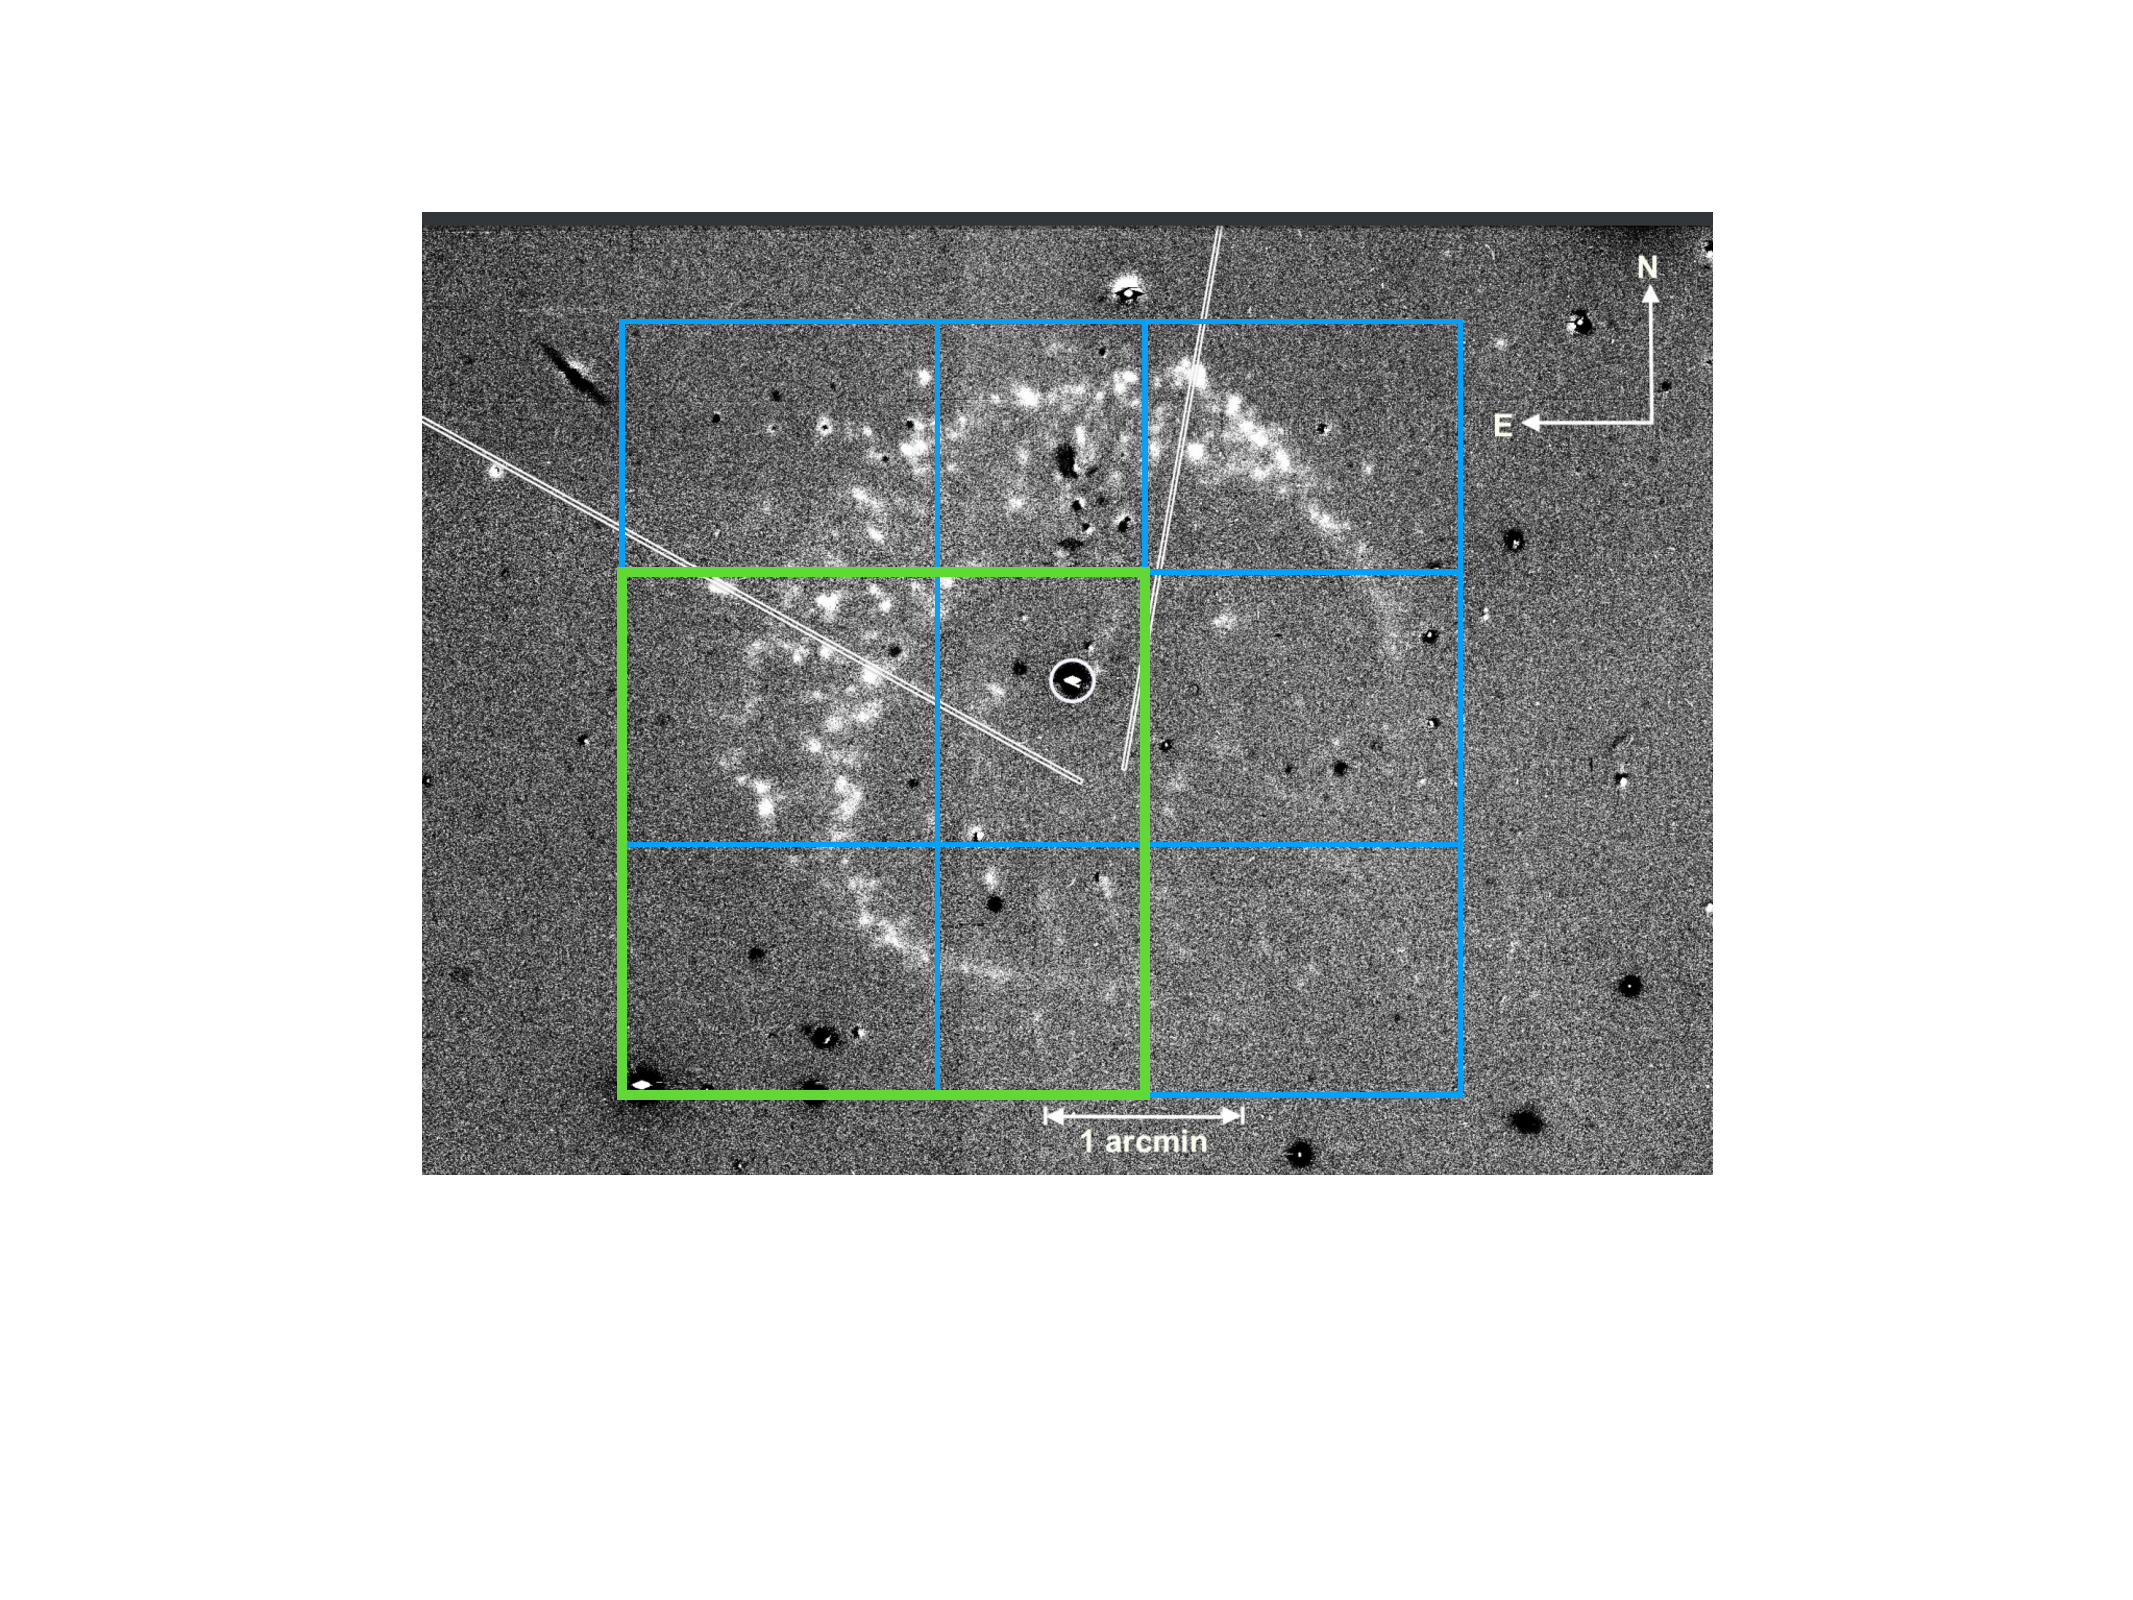
\includegraphics[width = \textwidth]{alma_proposal_template_v4/ATCnc.pdf} 
}
\caption{HST WFC3 FOV pointings for our observation plan. The green square represents the HST WFC3 FOV; we highlight a single pointing in a different color for clarity. We have a total of four different pointings, shown by the green and additional blue outlines. Each pointing will be observed twice for 500 seconds. The optical image of AT Cnc is from Shara et al. 2012 \cite{shara2012atcnc}.}
\label{fig:observationplan}
\end{center}
\end{figure}

\textbf{We need to add in references!}
\small{\bibliography{bibfile} }
\bibliographystyle{ieeetr}

\end{document}

